\documentclass[CS5104-Notes.tex]{subfiles}
\begin{document}

\section{Unsupervised learning}
In unsupervised learning, only the set of features $X_{1}, X_{2}, ..., X_{n}$ measure from $n$ data points are available, with no associated output variable $Y$. As such, the goal is no longer to try and predict, as there is no ``correct'' prediction. Instead, the goal is to discover interesting things about the data. For example is there an informative way to visualise the data? Can subgroups be discovered among the variables or data points?
\n
Unsupervised learning is often more challenging than supervised learning. It tends to be more subjective with no set goal for analysis. Furthermore, it can be hard to assess the results as there is no universal method for validation of the results. In fact, there is no way to check the result at all as there is no true answer. Despite these difficulties, unsupervised learning techniques are of growing importance, especially given today's data driven systems to try and gain a better understanding in some field or area.

\subsection{K-means clustering}
Clustering techniques is a very broad term refering to finding subgroups or \textbf{clusters} in a dataset. When data points are clustered, the goal is to partition them into distinct groups so that the data points within each group is similar to each other while points in different groups are quite different from each other. What is means to be similar or different must be more concretely defined for this.
\n
K-means clustering is a simple approach to partition the data set into $K$ distinct, non-overlapping clusters. The K-means algorithm assigns each data point to exactly one of the $K$ clusters. There are two properties which the $K$ clusters satisfy
\begin{enumerate}
\item $C_{1} \cup C_{2} \cup ... \cup C_{K} = \{1, ..., n\}$ - Each data point belongs to \textbf{at least} one of the $K$ clusters
\item $C_{k} \cap C_{k'} = \emptyset$ for all $k \neq k'$ - The clusters \textbf{do not} overlap, meaning no data point belongs to more than one cluster
\end{enumerate}
\begin{figure}[H]
  \centering
  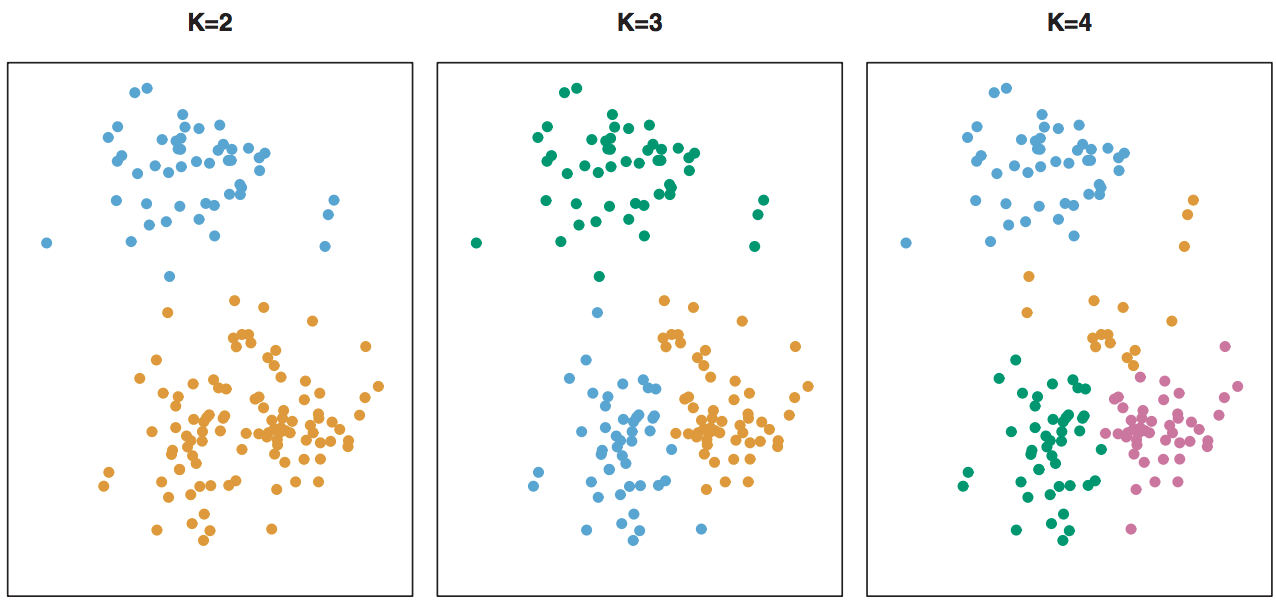
\includegraphics[width=0.9\textwidth, keepaspectratio]{imgs/different-k-means-clustering.png}
  \caption{Example of the same data set with a different value of $K$.}
\end{figure}

\subsubsection{Cost function}
The idea of a \textit{good} clustering is one for which the \textit{within-cluster variation} is as small as possible. This is a measure $W(C_{k})$ of the amount by which the data points within a cluster differ from each other. In other words, the optimisation problem becomes
\begin{equation}
\text{minimise } \Bigg\{\sum_{k=1}^{K}W(C_{k})\Bigg\}
\end{equation}
This means we wish to partition the observations into $K$ clusters such that the total variation within each cluster, summed over all clusters, is as small as possible. To do this, the measure $W(C_{k})$ must be defined. There are various ways to do this, and we shall look into the squared euclidean distance $||x||^{2}$.
\begin{align}
  W(C_{k}) &= \frac{1}{|C_{k}|}\sum_{i,i' \in C_{k}}\sum_{j=1}^{n}(x_{ij} - x_{i'j})^{2} \\
  W(C_{k}) &= \frac{1}{|C_{k}|}\sum_{i,i' \in C_{k}}\sum_{j=1}^{n}(x_{ij} - \mu_{c}(i))^{2}
\end{align}
The first equation defines the measure as the average distance of each point $x_{ij}$ to each other point $x_{i'j}$ while the second equation uses the centroid position $\mu_{c}(i)$ to which the data point $x_{i}$ is currently assigned to. This defines an average distance to the centroid.

\subsubsection{K-means clustering algorithm}
Given $K$ clusters with training data $x$ with $m$ examples:
\begin{algorithm}[H]
\begin{algorithmic}[1]
\Procedure{K-meansAlgorithm}{K}
  \State Randomly initialise $K$ cluster centroids $\mu_{1}, \mu_{2}, ..., \mu_{k}$
  \Repeat
    \For{$i = 1$ to $m$}
      \State Assign $x_{i}$ to cluster $c_{i}$ which minimises the equclidean distance to $\mu_{i}$
    \EndFor

    \For{$k = 1$ to $K$}
      \State $\mu_{k}$ = mean position of data points assigned to cluster $c_{k}$
    \EndFor
  \Until{Cluster assignments stop changing}
\EndProcedure
\end{algorithmic}
\caption{K-means algorithm for cluster initialisation and data point assignment.}
\end{algorithm}
The initial location of cluster centroids are randomly initialised to prevent any bias. Moreover, the algorithm can be repeated many times with randomly initialised centroid positions and the clustering with the lowest cost $W(C_{k})$ is the final clustering to pick. This is done because at the end of the algorithm, only a local minimum is found, the repetition leads to a higher chance of finding the global minimum.

\subsection{Principle component analysis}
Sometimes, instead of increasing the feature space with basis expansions, we wish to reduce the dimensionality of the input data. This could be done because of multiple reasons:
\begin{itemize}
\item Data compression to reduce the time to transfer the data and reduce the memory requirement
\item Reduces time needed for computation
\item Reduces amounts of redundant data
\end{itemize}
Principle component analysis is a way to reduce dimensionality automatically. It is an unsupervised technique as no output $Y$ is needed, but is often used as a way to produce derived variables for use in supervised learning.

\subsubsection{Principle components}
Suppose we are given a dataset with $n$ features $X_{1}, X_{2}, ..., X_{n}$ and $m$ data points, as part of the data visualisation and exploration stage, we may want to plot a two-dimensional scatterplot for each pair of features to find any correlations. However, there are $\frac{n(n-1)}{2}$ such scatterplots. If $n$ is large, it becomes less feasible to look at all of them. Furthermore, it is likely none of them will be informative as each only contain a small fraction of the total information present in the dataset. As a solution to this, we wish to find a lower-dimensional representation of the data that still captures as much information as possible so we can plot the data in this lower-dimensional space.
\n
PCA does exactly this by finding a low-dimensional representation of the dataset that contains as much information as possible. Note that mean normalisation and feature scaling should be performed \textit{before} applying PCA. 

\end{document}